%  Document Config
\documentclass[12pt]{diazessay}



\ksulogo{
    \begin{tikzpicture}[remember picture,overlay]
    \node[anchor=north west,yshift=-1.5pt,xshift=1pt]%
        at (current page.north west)
        {
\includegraphics[height=30mm]{Figures/KSU_logo.png}};
    \end{tikzpicture}
}

\school{King Saud University \\
College of Computer and Information Sciences\\
Computer Science Department}

\title{\textbf{Arabic Text Dialect Recognition}}

\logo{
    \begin{figure}[h]
        % \hskip-3.3cm
        \centering
        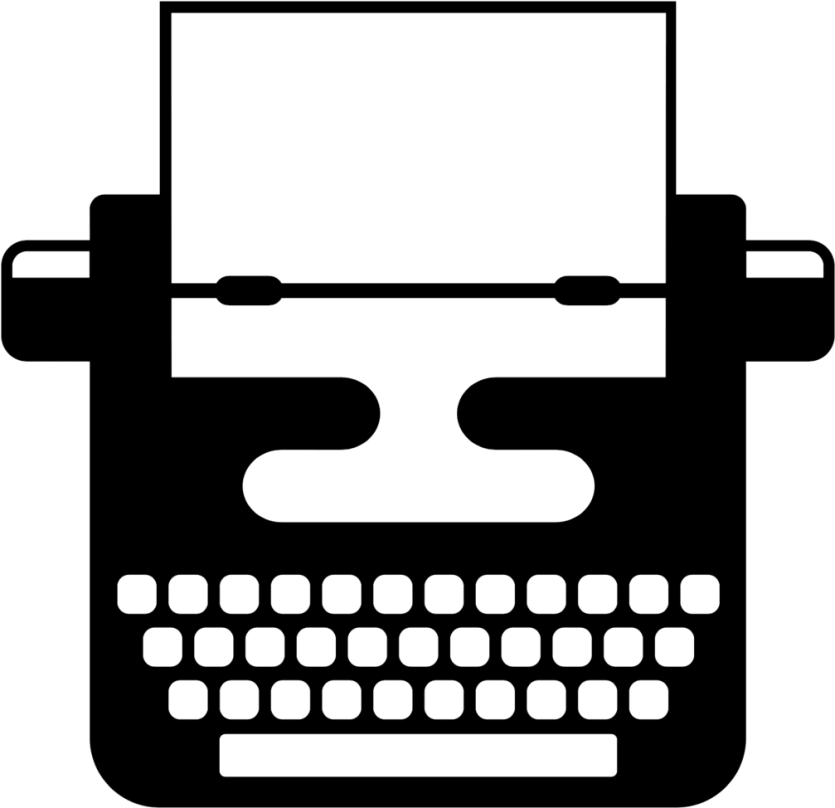
\includegraphics[scale=0.2]{Figures/best_project_logo.png}
    \end{figure}
}

\author{\textbf{Authors} \\ 
Mohand Al-Rasheed \hspace{15pt} 439101298\\
Khalid Albader \hspace{50pt}  439101990\\
Abdulrahman Alshawi \hspace{4pt}  439101980\\
Abdullah Alsuwailem \hspace{11pt}  439101690\\
Musaad Alqubayl \hspace{35pt}  439101884\\
} 
\supervisor{Dr. Nasser Alsadhan}

\date{Research project for the degree of Bachelor in Computer Science \\
First/Second Semester 1443 \\
Autumn/Spring 2021}

% Image config
\usepackage{graphicx}
\graphicspath{ {./Figures/} }

% Code config
\usepackage{listings}
\usepackage{color}

\definecolor{dkgreen}{rgb}{0,0.6,0}
\definecolor{gray}{rgb}{0.5,0.5,0.5}
\definecolor{mauve}{rgb}{0.58,0,0.82}
\definecolor{backcolour}{rgb}{0.99,0.99,0.99}


\lstset{frame=tb,
  language=Python,
  aboveskip=3mm,
  belowskip=3mm,
  showstringspaces=false,
  columns=flexible,
  basicstyle={\small\ttfamily},
  backgroundcolor=\color{backcolour},   
  numbers=left,
  numberstyle=\tiny\color{gray},
  keywordstyle=\color{blue},
  commentstyle=\color{dkgreen},
  stringstyle=\color{mauve},
  breaklines=True,
  breakatwhitespace=true,
  tabsize=1
}


% Section config
\usepackage{titlesec}
\usepackage{hyperref}

\titleclass{\subsubsubsection}{straight}[\subsection]

\newcounter{subsubsubsection}[subsubsection]
\renewcommand\thesubsubsubsection{\thesubsubsection.\arabic{subsubsubsection}}
\renewcommand\theparagraph{\thesubsubsubsection.\arabic{paragraph}} % optional; useful if paragraphs are to be numbered

\titleformat{\subsubsubsection}
  {\normalfont\normalsize\bfseries}{\thesubsubsubsection}{1em}{}
\titlespacing*{\subsubsubsection}
{0pt}{3.25ex plus 1ex minus .2ex}{1.5ex plus .2ex}

\makeatletter
\renewcommand\paragraph{\@startsection{paragraph}{5}{\z@}%
  {3.25ex \@plus1ex \@minus.2ex}%
  {-1em}%
  {\normalfont\normalsize\bfseries}}
\renewcommand\subparagraph{\@startsection{subparagraph}{6}{\parindent}%
  {3.25ex \@plus1ex \@minus .2ex}%
  {-1em}%
  {\normalfont\normalsize\bfseries}}
\def\toclevel@subsubsubsection{4}
\def\toclevel@paragraph{5}
\def\toclevel@paragraph{6}
\def\l@subsubsubsection{\@dottedtocline{4}{7em}{4em}}
\def\l@paragraph{\@dottedtocline{5}{10em}{5em}}
\def\l@subparagraph{\@dottedtocline{6}{14em}{6em}}
\makeatother

\setcounter{secnumdepth}{4}
\setcounter{tocdepth}{4}


\begin{document}


\maketitle 


%----------------------------------------------------------------------------------------
%	ESSAY BODY
%----------------------------------------------------------------------------------------

\tableofcontents

\cleardoublepage

\addcontentsline{toc}{section}{Acknowledgements}
\section*{Acknowledgements}
We would like to express our great gratitude to Dr. Nasser Alsadhan for his valuable suggestions. and his aid throughout the writing of this report. His willingness to give his time so generously has been very much appreciated.

\addcontentsline{toc}{section}{English Abstract}
\section*{English Abstract}
The Arabic language is one of the oldest languages widely used today, and as a result of that, many Arabic speaking regions have formed dialects exclusive to their own. For example, many countries surrounding the Arabic Gulf have formed a dialect different to countries in the Levantine region. We intend on identifying and systematically determining the dialect of a piece of text. 

 This research has many applications in Arabic text analysis, such as helping in identifying the regions customers most often come from by analyzing a product’s reviews and comments and breaking them down by region, which provides useful intel for a business. It also helps in narrowing the nationality of an anonymous writer of a piece of text by predicting their region.
One of the major challenges in dialect recognition is dividing data into classes of dialects. Saudi Arabia and the UAE have dialects that differ widely from each other when solely considered, though they feel very similar in comparison to a Levantine dialect. The researchers will determine a classification easy enough for a machine to detect, but sophisticated enough to be useful. 

We intend to build a machine learning powered classifier that distinguishes between a set number of different Arabic dialects (e.g. Egyptian, Levantine, Gulf, etc.) when given a piece of text. We’ll use state of the art technologies in the field of NLP (natural language processing) in order to train an effective classifier that understands the differences between dialects.


\addcontentsline{toc}{section}{Arabic Abstract}
\section*{Arabic Abstract}
\begin{RLtext}
اللغة العربية من أقدم اللغات المستخدمة بكثرة حاليا، ونتيجة لذلك، الكثير من المناطق المتحدثة للعربية أنشأت لهجات مخصصة بمناطقهم. فعلى سبيل المثال، الكثير من المناطق المجاورة للخليج العربي تتحدث لهجة مختلفة بشدة عن لهجات المناطق الشامية. يعتزم الباحثون على أتمتة عملية التعرف على اللهجات من خلال تحليل قطعة من النص.

البحث له العديد من التطبيقات، وأهمها هو في تحليل النصوص العربية، فمثلا استخدامه في التعرف على مناطق عملاء جهة معينة عن طريق تحليل التقاييم والتعليقات المضافة على منتجاتهم، مما يمكن الجهة على التعرف على عملائهم بشكل أدق. كذلك يمكن استخدامه للتنبؤ بمنشأ مرسل رسالة مجهولة عن طريق التعرف على منطقة نشأته.

من أهم التحديات في تصنيف اللهجات هي تقسيم البيانات لأصناف من اللهجات. فعلى سبيل المثال، المملكة العربية السعودية والإمارات العربية المتحدة يتحدثون بلهجات مختلفة إذا حصرنا النظر عليهم، ولكن يشبهون بعض حين تتم مقارنتهم مع اللهجات الشامية. سيختار الباحثون مجموعة مناسبة من اللهجات حيث تكون سهلة للنظام في التعرف عليها، ولكن معقدة كفاية لكي تكون مفيدة.

في هذا المشروع ننوي بناء مصنف (\LR{classifier}) مدعوم بتقنيات تعلم الآلة لكي يصنف ما بين مجموعة من اللهجات المحددة (مثل اللهجة المصرية، والشامية، والخليجية، وغيرها) إذا أعطي قطعة من النص. سيستخدم الباحثون أحدث التقنيات في مجال تحليل اللغات الطبيعية (\LR{NLP}) لكي يدربوا مصنف فعال، يفرق بين اللهجات العربية.
\end{RLtext}


\section{Introduction}
    As languages develop across regions far apart from each other dialects begin to take shape, machine learning researchers became interested in classifying text in some language to it's proper dialect. This is because its connected to more insightful text analysis.
    
    A dialect is the variation of a language in grammar, pronunciation and vocabulary. Every individual has their own way of talking that is affected by dialect, accent, background and many other factors\cite{10.5555/2126240}. The Arabic language has a variety of dialects throughout the Arabic world, dialects could differ not only across countries but also in the same country or even city. Arabic dialects differ from one another in pronunciation and vocabulary, different dialects have different words or different variations of a word that could refer to the same meaning, which sometimes make it a bit difficult to understand each other, and it can make it harder for non-Arabic speakers who are trying to learn Arabic.
    
    Machine Learning is a field of study that is concerned with developing algorithms that utilize data with the intent of solving tasks traditional methods cannot solve, in a way similar to how humans approach complex problems\cite{ibm_cloud_education_2020}. It is a rapidly growing field, many countries are racing each other to adapt machine learning technologies and develop smart and automated systems, applications, and adapt them into our daily lives as well as numerous varieties of fields that could benefit from them. Natural language processing, abbreviated as \textit{NLP} is a branch of machine learning that is primarily focused on analyzing text. Numerous companies are racing to develop programs that utilize NLP to analyze user behaviour. One of the difficulties facing companies developing using NLP for Arabic speakers is the numerous varieties of dialects in Arabic.


    \subsection{Problem statement}
    
    Dialects are formed mainly due to regional separation between the Arab world. This separation reduces interaction between different regions, and as a result of that, many Arabic speaking regions have formed dialects exclusive to their own. For example, many countries surrounding the Arabic Gulf have formed a dialect different to countries in the Levantine region. The research’s main problem is how to identify and predict dialect types from text.

 
    \begin{figure}[h]
        % \hskip-3.3cm
        \centering
        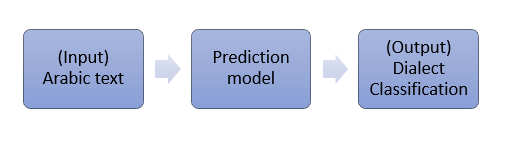
\includegraphics[scale=0.7]{Figures/problem_statment.png}
        \caption{Illustration of the problem}
        \label{fig:cmp}
    \end{figure}
        
    
    \subsection{Goals and objectives}
    
    The goal of this research is to analyze and understand Arabic text to classify the dialect of any piece of Arabic text.
    The objective is to implement the most appropriate state of the art NLP model that helps in achieving the best possible accuracy which correlates to correctly classifying what dialect the text is from.

    \subsection{Proposed solution}
    This research will contribute in solving Arabic dialect detection by using one of the latest advancements in the field of natural language processing.
    
    
    \subsection{Research scope}
    The scope of this research is mainly focused about analyzing, preprocessing and modeling a state of the art NLP model to classify Arabic text into a set of dialects. 


\section{Background}


    \subsection{Natural language processing}
        “Natural Language Processing is a theoretically motivated range of computational techniques for
        analyzing and representing naturally occurring texts at one or more levels of linguistic analysis for the purpose of achieving human-like language processing for a range of tasks or applications.” \cite{natural_language_processing_book}. The field of NLP is an active area of research and development solely for the purpose of computerizing the process of analyzing written/spoken text in a human-like way.
        
        In recent years NLP has become an essential part for many technologies that are relevant today. Companies are taking advantage of the abundance of data that is flooding the internet every day and are developing numerous NLP technologies and applications that we use everyday.
        
        Human languages are surprisingly complex and ambiguous in nature, there are languages that are easier to process for computers than others due to various reasons. German for example relies heavily on morphology and compositional word-building that aids in generalizing to unseen words\cite{Felipe_Geraldo}. However, there has been continuous advancements done on computational techniques that will try to solve challenges around the ambiguity of languages.
    
        
        \subsubsection{Preprocessing}
            Preprocessing refers to the manipulation of raw data to format it in a way that is easier for computers to process and analyze. It is a technique that is crucial for any NLP task to perform well, it can directly impact the accuracy and performance of any kind of task performed on it. It is the first step taken for any NLP task. Some operations of preprocessing include, \emph{normalization} of data, \emph{segmentation} of data, \emph{tokenization} of text, \emph{stemming} of words and \emph{noise removal}. When dealing with Arabic text usually the first step is filtering out non-Arabic content from text especially when you are getting the content from social media.
            
            In this section we will discuss the most important steps in preprocessing, such as tokenization and converting text to embeddings.


            \subsubsubsection{Tokenization} \label{txt:tokenization_section}
            Tokenization is the process of breaking down input text into smaller components called tokens so that its easily analyzable for computers. It is an important step in preprocessing text for any NLP task. There are several methods for performing tokenization, such as white tokenization, subword tokenization and others. White space tokenization breaks sentences into words that we call tokens, while this is useful for languages like English and French, it is needed to perform some additional steps for languages like Chinese and Japanese where words are not separated by spaces. While subword tokenization breaks down words into different tokens, so for example, "Unfriendly" is broken down to "Un", "friend" and "ly" \cite{subword_tokenization}.
            
            Tokenization also has limitations for the Arabic language, owing to the complexity of the language, words like "\RL{عقد}" and "\RL{جد}" depending on the context or pronunciation could lead to different meanings, So the word
            "\RL{عقَدَ}".
            means to tie, which is different from
            "\RL{عَقَّدَ}".
            which means to over-complicate.
            Also there are huge differences in formal and informal Arabic (more on that in section \ref{txt:thearabiclanguage}), as well as different dialects having vastly different sentence structure. and not just in Arabic this is also true for most languages, and that is one of the challenges of tokenization.
    
            
            \subsubsubsection{Word embedding}
            \begin{figure}[h]
                % \hskip-3.3cm
                \centering
                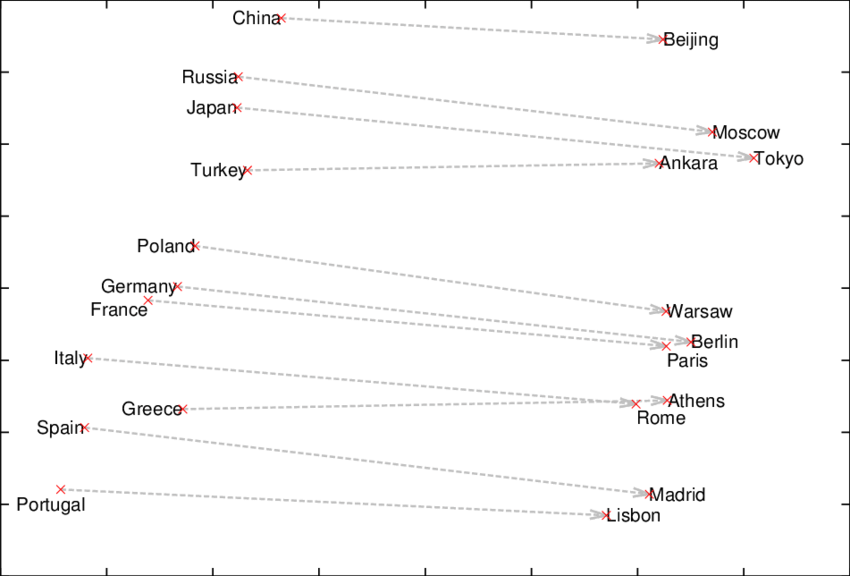
\includegraphics[scale=0.42]{Figures/embeddings_fig.png}
                \caption{Country and capital vectors projected by PCA \cite{PCA_article}}
                \label{fig:wordembedding}
            \end{figure}
            
            Computers can’t understand natural language, so in order to make computers understand it we have to create a representation for a language that a computer can process, and that is what word embedding do. Word embedding is a representation of words that encodes the semantic meaning of words in vectors, such that words that are similar in meaning are probably going to be close in vector space \cite{jurafsky_martin_2000}. There are several word embedding models, and generally all models share the concept of context to determine how close are words to each other, “You shall know a word by the company it keeps!” (Firth, J. R. 1957:11). Figure \ref{fig:wordembedding} shows a model that learnt the relationships between countries and their capitals without information of what a capital city means.
    
        
    \subsection{Neural networks}
        Neural networks are a sub-field of machine learning, and also the parent field of deep learning. Neural networks are made up of layers of neurons and work like interconnected nodes inspired by the neurons inside the brain. By taking in data, they are able to recognize hidden patterns and correlations in unprocessed data and use said patterns to cluster, classify and predict the data, among other applications.
        
        A typical neural network architecture contains the following:
        \begin{enumerate}
            \item Input layer: takes the initial data.
            \item Hidden layer(s): a layer, or more, placed between input and output which captures the non-linearity of the data.
            \item Output layer: produce the outcome of the prediction.
        \end{enumerate}
        
        \begin{figure}[h]
            % \hskip-3.3cm
            \centering
            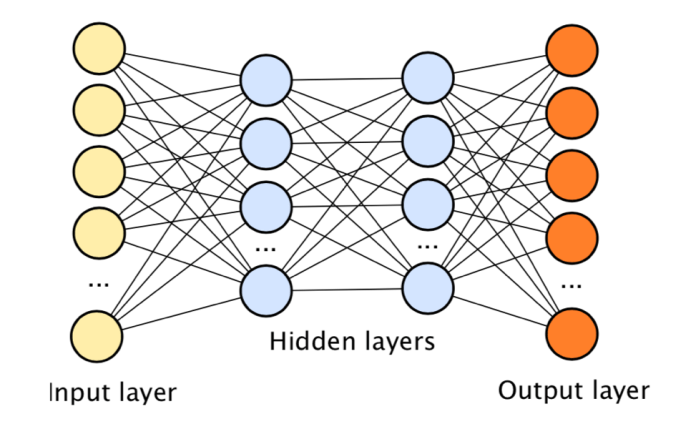
\includegraphics[scale=0.5]{Figures/neural networks.png}
            \caption{Neural networks architecture \cite{marcus2018deep}}
            \label{fig:cmp}
        \end{figure}
        
        Neural networks also are ideally fitted to assist humans solve complicated issues in real-life situations. They can examine and model the relationships among inputs and outputs which can be nonlinear and complicated as well as make generalizations and inferences,
        
        
        % \subsubsection{Neural networks in natural language processing}
        Neural networks are now prevalent in NLP such text classification (which is the objective of this research), machine translation, semantic parsing, which extracts useful bits of information in a large text, and many more.
        
        % A great amount of NLP based applications (e.g., sentiment analysis, text classification, etc...) depend on language models. which define a probability distribution over sequences of words, characters or bytes in a natural language Different pre-trained language models have been proposed to address various domain-specific problems, one such model is BERT. 
        %%%%%%%%%%%%%%%%%%%%% Great summary of language representation, I think we might need to write it in the methodology section
        

        \subsubsection{Deep learning}
        Deep learning is a machine learning model that utilizes large neural networks. deep learning have dramatically developed the state-of-the-art in speech recognition, object detection and a number of different domains along with genomics and drug discovery\cite{Hinton}. % Deep learning discovers complex patterns in massive data units to signify how a machine must change its inner parameters which are used to compute the illustration in every layer from the representation withinside the previous layer.
        
        While deep learning isn't accurately defined, what differentiates deep learning models from other neural networks models is primarily the number of layers and the time it takes to train. An example of a deep learning model is \emph{Convolutional Neural Networks} (CNNs) which are commonly used with images. Extracting meaning from a 2D structure such as images can be quite hard for traditional machine learning algorithms because of the inherent complexity of the patterns in image data, this complexity can be tackled by deep learning models though they require a large number of layers as well as long training time.
        
         
        \subsubsection{Transformers} \label{txt:transformers_section}
        Since its introduction in 2017 by the google research team, its rapid growth dominated the NLP field and became a standard for any encoder/decoder model today\cite{wolf-etal-2020-transformers}. the transformer takes advantage of parallelization unlike Recurrent Neural Networks (RNNs), which process data in a sequential order, which is computationally more expensive compared to the transformer model\cite{46201}. In a high level overview, its model architecture can be divided into two major components, an encoder and a decoder. An encoder maps the input sequence to a numeric representation that holds information about the input sequence, the decoder given the output of the encoder generates a sequence of symbols one element at a time, the model consumes the previously generated symbols as additional input when generating the next\cite{46201}.

        There are many models used today that are built on the transformer architecture especially in NLP, for example, \emph{Bidirectional Encoder Representations from Transformers} (BERT) is a popular transformer-based model. Also, OpenAI's \emph{Generative Pre-trained Transformer} (GPT) models are transformer models that garnered wide attention for being excellent in imitating human produced text.
        

    \subsection{Dialect prediction approaches}
        One can approach the problem of dialect prediction in a number of ways, We will define and discuss some different dialect recognition approaches that differ in how they work.

        
        \subsubsection{Rule-based approach}
        Rule-based approach relies in written curated instructions made by humans to identify selected parts of the text that match a certain logic or found in dictionaries, a popular example in text classifications is to count the number of each word that relate to a category and the highest word count for a category classifies the text in that category. 
        
        Another example would be the Lexical Functional Grammar (LFG). "The LFG system incorporates a richly annotated lexicon containing functional and semantic information."\cite{hassan_2010}.

        
        \subsubsection{Automatic machine-learning approach} \label{txt:simple_voting}
        The automatic approach in dialect recognition is based on machine learning, where it tries to build a statistical model that learns by analysing the training data after choosing an appropriate algorithm and applying NLP techniques. The most prominent algorithms in text classification would be support vector machines (SVMs), Naïve Bayes and deep learning methods.
        
        
        \subsubsection{Hybrid approach}
        "Hybrid systems combine a machine learning-trained base classifier with a rule-based system, used to further improve the results. These hybrid systems can be easily fine-tuned by adding specific rules for those conflicting tags that haven’t been correctly modeled by the base classifier."\cite{monkey_learn_NLP}
        
        
    \subsection{Performance metrics}
    In binary\footnote{We can use precision and recall in multiclass classification by considering one class, \(A\), at a time and lumping all other classes as \(not A\)} classification problems, we can test the performance of our results by matching the output of our model, the predicted label, to the real label in our data. This measure is known as the \emph{accuracy} of our model according to the data. However there are more sophisticated measures that one can observe. We'll talk about two of those measure, mainly \emph{precision} and \emph{recall}.
    
    First, we must define 4 quantities, \textbf{True Positive}, abbreviated \(TP\) consists of \emph{true} which refers to the data belonging to class 1, while \emph{positive} refers to the model's prediction belonging to class 1. And \textbf{False Negative} is similar to \(TP\) but in the context of class 0. We can mix and match \(T\), \(F\), \(P\) and \(N\) to get 4 different quantities.
    
    Here we define precision and recall in the following way:
    
    \[Precision = TP / (TP + FP)\]
    
    \[Recall = TP / (TP + FN)\]
    
    We can tweak the model's threshold of classification in order to achieve a different Precision and Recall metrics


\section{Literature review}
The discussed problem in this research has been tackled by many researchers over the years with varying results. in this section we intend to highlight the most important results regarding the Arabic language, the Arabic corpora and dialect classification methods that have been concluded from past research.
    
    
    \subsection{The Arabic language} \label{txt:thearabiclanguage}
    Arabic speakers often use Modern Standard Arabic (\emph{MSA}) when they're in a formal setting such as reading the news, though they have a regional dialect that they talk with in informal settings. In this section we'll detail the work made to document and break down different dialects into regions they belong to. 
        
        
        \subsubsection{Arabic dialects}
        Dividing Arabic into different dialects is not a standardized task as dialects shift and change depending on the time and how much precision we intend to administer in our breakdown. Researchers working on this problem have found various breakdowns that we'll discuss.
        
        Habash has suggested the following breakdown, while adding "and should not be taken to mean that all members of any dialect group are completely homogenous linguistically" \cite{habash}.
        \begin{enumerate}
            \item Egyptian Arabic (EGY) which spans Eygpt and Sudan
            \item  Gulf Arabic (GLF) which spans the Arabic peninsula, Habash adds "although there is a wide range of sub-dialects within it." And "Omani Arabic is included some times."
            \item Levantine Arabic (LEV) which spans the Levantine region
            \item "North African (Maghrebi) Arabic (Mag) covers the dialects of Morocco, Algeria, Tunisia and Mauritania. Libyan Arabic is sometimes included." \footnote{Many other researchers abbreviate North African dialects as "NOR"}
            \item "Iraqi Arabic (IRQ) has elements of both Levantine and Gulf"
            \item "Yemenite Arabic (Yem) is often considered its own class"
        \end{enumerate}
        
        \begin{figure}[h]
            % \hskip-3.3cm
            \centering
            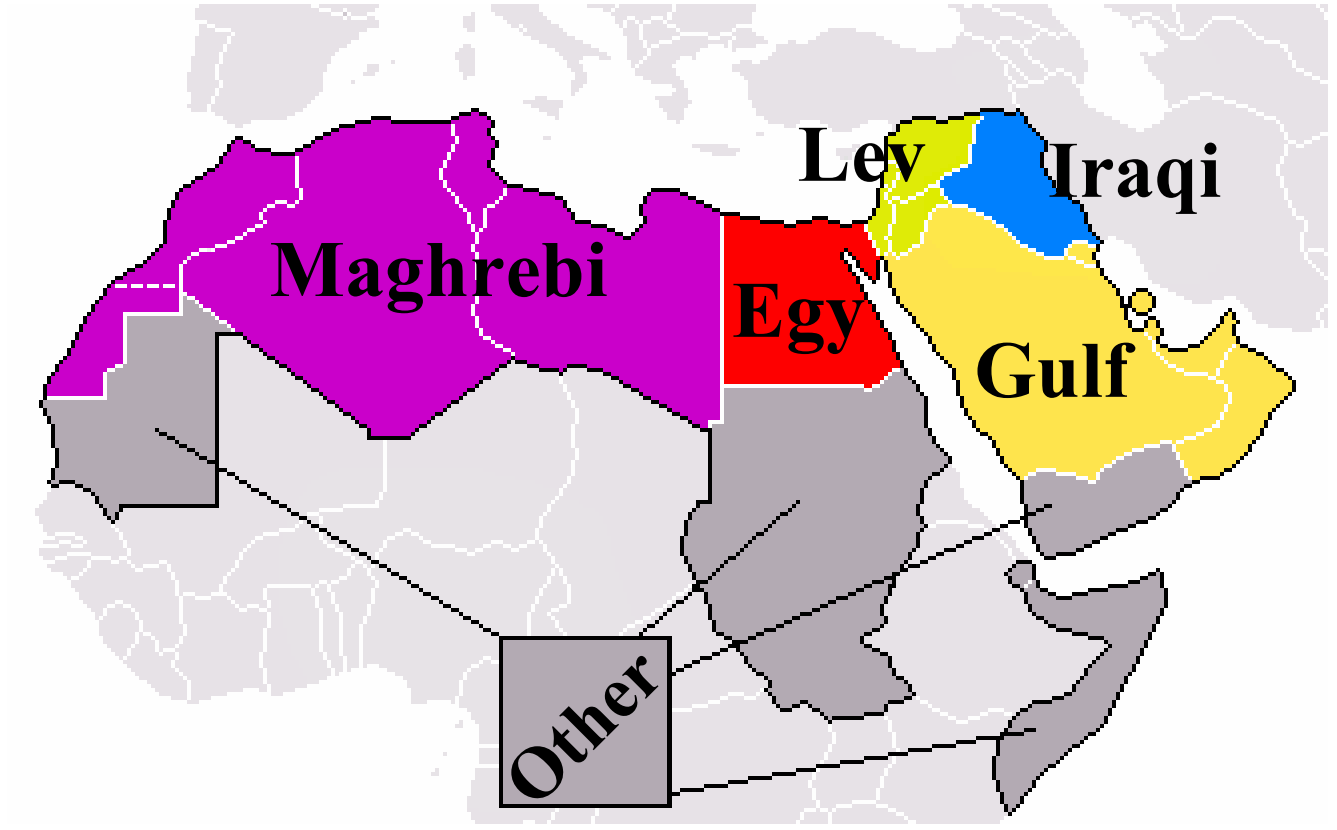
\includegraphics[scale=0.2]{Figures/Zaidan and Burch dialect breakdown.png}
            \caption{Zaidan and Callison-Burch (2011) gave a similar breakdown\cite{zaidan_burch} to Habash's}
            \label{fig:cmp}
        \end{figure}
        
        Alshutayri also gave a similar breakdown, which is GLF (including Oman), EGY, LEV, NOR (which includes Morocco, Algeria, Tunisia and Libya) and IRQ. Although the breakdown is somewhat general and imprecise, its general enough to be useful in data collection and in classification\cite{alshutayri}.
        
        
    \subsection{Existing Arabic text corpora}
    The problem of dialect classification has been studied in the past with many studies building their own corpora, here we'll examine the most prominent of corpora.
    
    In 2015 Shoufan and Alameri conducted a literature review, in which they summarised the advancements in NLP for dialectal Arabic in the following comprehensive table\cite{shoufan_alameri_2015_natural}. Bear in mind that the table includes more than text analysis and also includes speech analysis.
    
    \clearpage
    \begin{table}[h]
        \hskip-3cm
        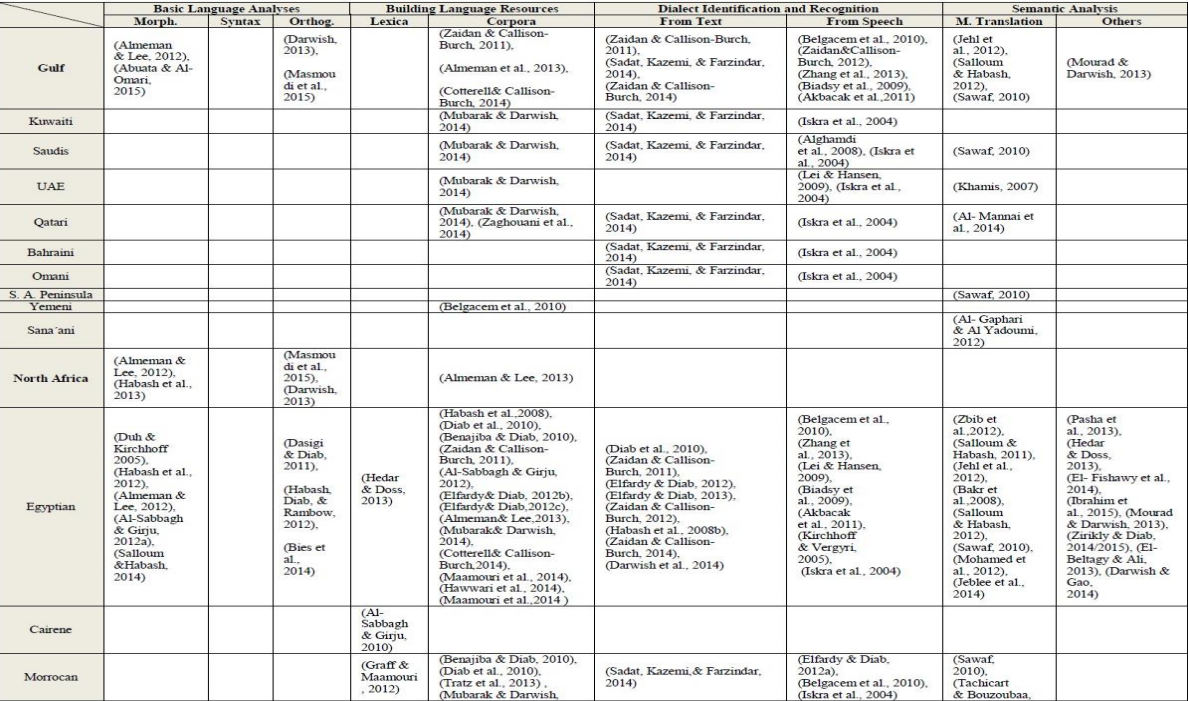
\includegraphics[scale=0.45]{Figures/past_word_1.png}
        \caption{Dialectical Arabic NLP- Literature Overview\cite{shoufan_alameri_2015_natural}}
        \label{fig:cmp}
    \end{table}
    
    \clearpage
    \begin{table}[h]
        \hskip-3cm
        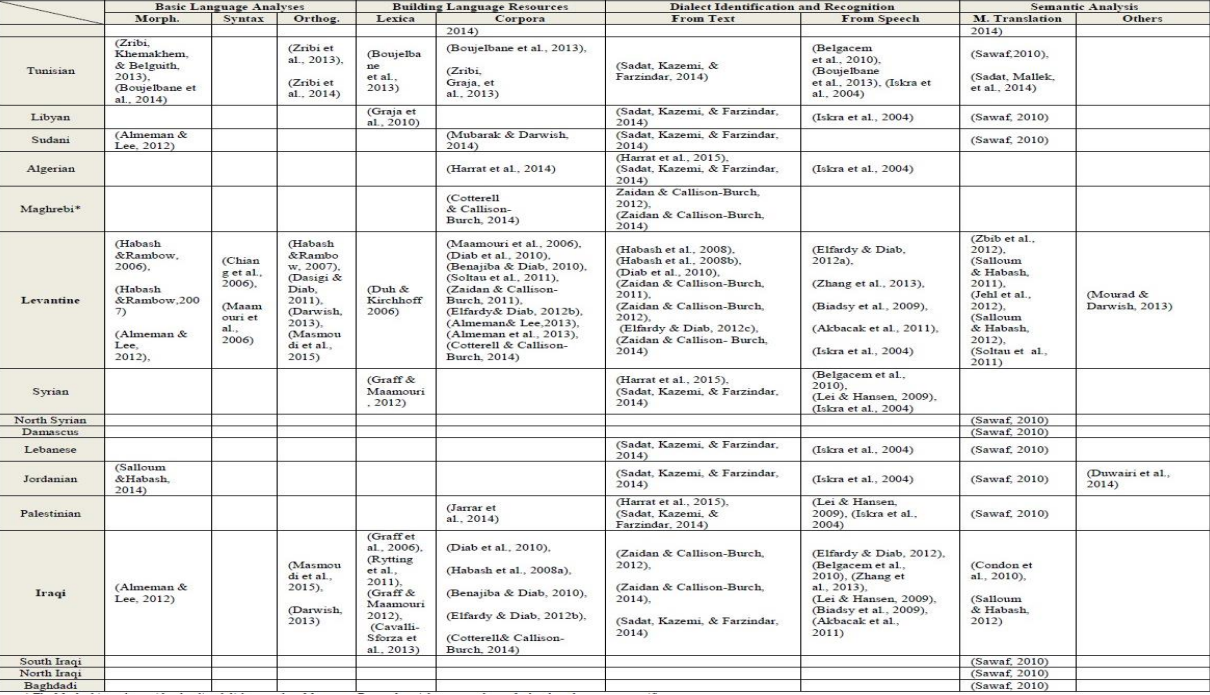
\includegraphics[scale=0.45]{Figures/past_work_2.png}
        \caption{Dialectical Arabic NLP- Literature Overview\cite{shoufan_alameri_2015_natural}}
        \label{fig:cmp}
    \end{table}
    \clearpage
    
    
    The most prominent corpora collected is the Arabic Online Commentary (AOC) dataset which gathered millions of comments from three newspapers\cite{zaidan_burch}\label{txt:aoc}.
    
    Though the AOC dataset was big enough, it was not annotated fully, which might harm a predicting model's results. There has been work in creating an annotated dataset built from the AOC dataset alongside North African dialectical data collected from the Tunisian Arabic Corpus\footnote{http://www.tunisiya.org/}. Then the researchers annoatated the collected data by using Amazon's \emph{Mechanical Turk} (MTURK), which hires online annotators\cite{el_haj_etal_2018_arabic}.
     
    Another improvment of the AOC dataset came from Cotterell and Callison-Burch, in which they extended the AOC newpaper dataset to include about 550K words from 5 newspapers "\textbf{Al-Youm Al-Sabe’}, a Saudi-Arabian newspaper \textbf{Al-Riyadh}, a Jordanian newspaper \textbf{Al-Ghad}, an Algerian newspaper, \textbf{Ech Chorouk El Youmi} and an Iraqi newspaper \textbf{Al-Wefaq}.". As well as 660k words scraped from twitter tweets. After collecting the extended dataset, they manually annotated them using Amazon's Mechnical Turk\cite{cotterell-callison-burch-2014-multi}.
     
    There has been work in using social media as a valid source of dialectic data, creating the Social Media Arabic Dialect Corpus (SMADC) dataset, which scraped and annotated data from Twitter and Facebook\cite{alshutayri_inproceedings}.\label{txt:SMADC_talk}
    
    Another dataset is the The Dialectal Arabic Tweets (DART), which manually annotated over 25k tweets in Maghrebi, Egyptian, Levantine, Iraqi, and Gulf\cite{alsarsour-etal-2018-dart}.
     
     
    \subsection{Dialect classification results}
    There has been many attempts in solving the problem of this research, many of which use similar strategies. In this section we'll review the highlights of past literature's results.
    
    % https://www.cs.jhu.edu/~ccb/publications/arabic-dialect-corpus.pdf
    Zaidan-Burch, the researchers behind the AOC dataset, mentioned in section \ref{txt:aoc} the results they found as well as their methodology. They used a "SRILM toolkit to build word trigram models, with modified Kneser-Ney as a smoothing method, and report the results of 10-fold cross validation"\footnote{The SRI Language Modeling Toolkit (SRILM) is a toolkit for building statistical language models}. They have achieved an accuracy of 69.4\% at classifying "MSA vs. LEV vs. GLF vs. EGY"\cite{zaidan_burch}.
    
    Cotterell-Burch have extended the AOC data, also mentioned in section \ref{txt:aoc} and trained using two algorithms, SVM and Naive Bayes using unigram, bigram and trigram features\cite{cotterell-callison-burch-2014-multi}. The results are displayed in figure \ref{fig:extended_aoc_results}.
    
    \begin{figure}[h]
        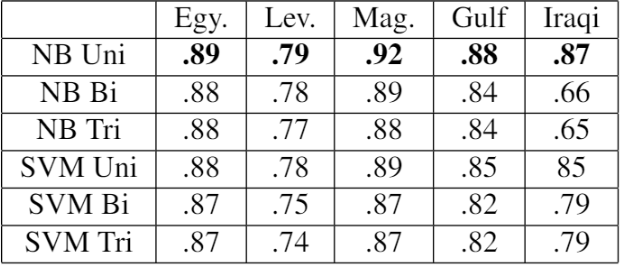
\includegraphics[scale=0.6]{Figures/results_extended_AOC.png}
        \caption{"Experiments on newspaper commentary data (accuracy reported)."\cite{cotterell-callison-burch-2014-multi}}
        \label{fig:extended_aoc_results}
    \end{figure}
    
    Alshutayri used the SMADC dataset to classify dialects to GLF, NOR, LEV, EGY and IRQ. They used Sequential Minimal Optimization (SMO) algorithm with multinomial Naive Bayes (MNB) with different tokenizers, run via the data analysis tool WEKA to achieve an accuracy of 60.68\%\cite{alshutayri}.
    
    Alshutayri have also tried lexical methods. One of which is simple voting, which was described in section \ref{txt:simple_voting}. Using the SMADC dataset, the researcher achieved an accuracy of 69.19\% The researcher also experimented with weighted voting, filtering based on MSA words and more\cite{alshutayri}.
    
    \begin{figure}[h]
        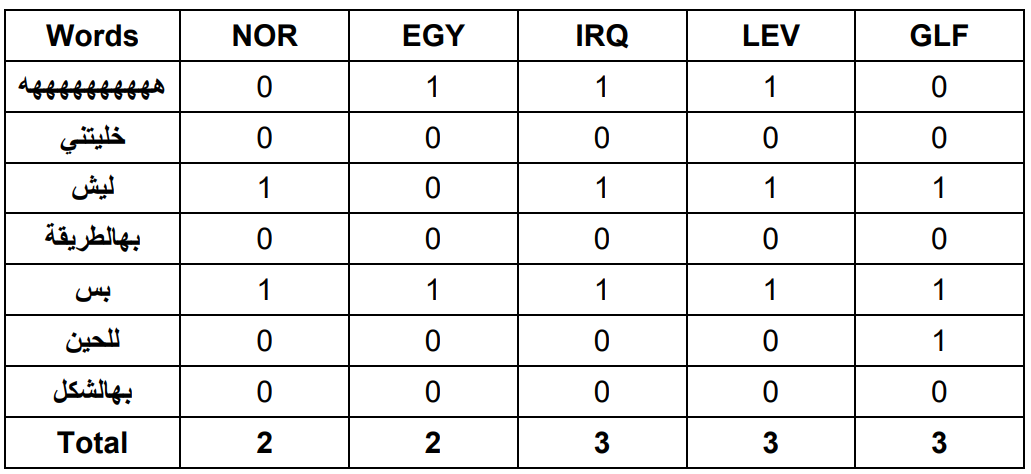
\includegraphics[scale=0.35]{Figures/smadc_simple_voting.png}
        \caption{Simple voting matrix representation of \RL{ههههههههههه خليتني ليش بهالطريقة بس للحين بهالشكل}\cite{alshutayri}}
    \end{figure}
        
        
        \subsubsection{Deep learning dialect classification results}
        Most of the research around dialect classification uses traditional text classification methods and deep learning methods are scarcely used, however, the surge of deep learning research has reinvigorated the interest in deep learning text classification.
        
        Elaraby and Abdul-Mageed have used many different algorithms including deep learning algorithms such as CNN, CLSTM, LSTM, BiLSTM, BiGRU and Attention BiLSTM which they explain in their paper as well as traditional classifiers such as SVMs, Naive Bayes and others\cite{elaraby-abdul-mageed-2018-deep}.
        
        On the AOC dataset Elaraby and Abdul-Mageed used this dialect split "MSA vs. Egyptian vs. Gulf vs. Levantine" to obtain an accuracy of 82.45\% using the Attention BiLSTM with Abdul-Mageed, et al. embeddings\cite{elaraby-abdul-mageed-2018-deep}.
        
        It's also noteable that the traditional classifiers won over deep learning classifiers only on the "EGY, GLF, and LEV" three way classification split\cite{elaraby-abdul-mageed-2018-deep}.
        
    
    \section{Methodology}
        % big graph, detailed and has example input and example output (use something like drawio)
        
        % Hawzen Domain
            \subsection{The SMADC dataset}
            In this research we'll be using the Social Media Arabic Dialect Corpus (\emph{SMADC}) dataset that we talked about in section \ref{txt:SMADC_talk}. We'll briefly note important details about its collection, filtration and annotation.
            
                \subsubsection{Collection}
                SMADC's corpus is collected from three different sources, Facebook, Twitter and online newspapers. We'll briefly go over the details of collection for each source. 
                
                For Twitter documents, the researchers collected 210,915 tweets, then proceeded to label tweets based on the existence of pre-defined seed words and the location of the tweet's sender as well as the Geo-location of the tweet. For Facebook documents, the researches scraped 2,888,788 comments from 422,070 Facebook posts. They annotated the comments based on the country of the account the post was from. For online newspapers, the researchers collected 10,096 comments from 25 newspapers and were automatically labeled based on the newspaper's origin country.\cite{alshutayri}
                
                Though this simple annotation was manually checked and corrected if it were to be false, we'll discuss more of that in section \ref{txt:annotation}.
                
                \subsubsection{Filteration}
                The researchers filtered Facebook and Twitter documents automatically by removing hashtags, emojies, redundant characters and so on. They also found some difficulties making sure that their dataset is polished. They started filtering the noises of their dataset, to assure that it will improve the accuracy. Notable noises such as writing a nationality that conflicts with the label, non-Arabic characters, spelling mistakes, etc.\cite{alshutayri}
        
                \begin{table}[h]
                     % \hskip-3.3cm
                    \centering
                    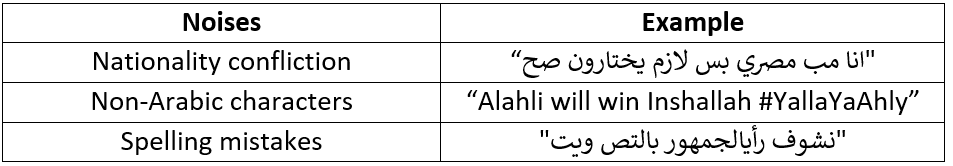
\includegraphics[scale=0.80]{Figures/noises_table.PNG}
                    \caption{Different noises that got filtered}
                    \label{tbl:noises}
                \end{table}
                
                \subsubsection{Annotation} 
                \label{txt:annotation}    
                After automatically annotating the documents in the way we described earlier, the researcher has used novel manual annotation techniques to annotate a part of the dataset. They had created an interactive online quiz where users would log in and manually annotate a number documents. Control documents was placed to check if the user is not randomly choosing options, and annotation conflicts were resolved by choosing majority voting. Resulting in 24,060 manually annotated documents. \cite{alshutayri}
                
        
        % D7 Domain
        
            % Moon
            % Arrow
            % Looking
            % Leading
            % Creating
            
            % Doing
            % Embedding
            % Synthesising
            % Nurturing
            % Tempting
            
            % 0
            
            % Read first character of every word
        
        \subsection{Preprocessing}
        We used preprocessing techniques that help in transforming the data to a represntation the model understands, like tokenization and segmentation which we will discuss in this section.
        
            \subsubsection{Tokenization}
            As we discussed in section \ref{txt:tokenization_section} tokenization is an essential task for NLP problems. We'll be using tokenization to clean our dataset and transform it to be ready for classification.
            
            While tokenizing our dataset we'll filter any non-Arabic tokens that hasn't been already filtered, such as text from other languages, emojies and other symbols. We also will remove and Arabic diacritics such as fatha, damma, kasra and so on. so the following word \RL{مُذَكِّراتِهِ} 
            will be transformed to \RL{مذكراته}, this should help the model group similar words, albeit lost a bit of accuracy.
            
            \subsubsection{Segmentation}
            Word segmentation is a preprocessing step for many NLP tasks, especially when dealing with rich languages like Arabic.
            
            Arabic word segmentation works by separating the suffixes and prefixes attached to any given word, a simple example can be seen with the word \RL{العربية} which can be segmented to \RL{ال + عربي + ة}, in this example we can see that the prefix in this word is \RL{ال} and the suffix is \RL{ة} and the stemmed word is \RL{عربي}, segmentation has shown to have significant impact in many NLP application such as context understanding, because it gives more information to the model. Another more sophisticated example is shown in Figure \ref{fig:arabic_segmentation}
            
            \begin{figure}[h]
                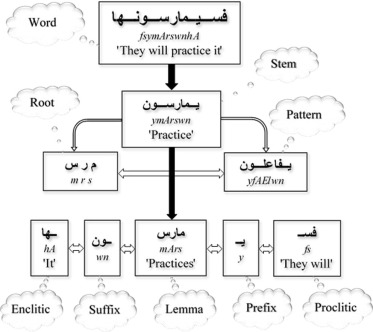
\includegraphics[scale=1]{Figures/arabic_segmentation.png}
                \caption{Example of Arabic word segmentation.\cite{arabic_segmentation}}
                \label{fig:arabic_segmentation}
            \end{figure}
            
            % The researchers didn't have to make a segmentation function because we made use of the segmentation function that is internally integrated in AraBERT which uses Farasa segmenter\cite{Farasa}.
            % Lets mention this in the implementation, actually
        
        % Hawzen Domain
        \subsection{BERT}
            \subsubsection{BERT overview}
            After the release of the transformer model that we talked about in section \ref{txt:transformers_section} in 2018 Google research released the Bidirectional Encoder Representations from Transformers, \emph{BERT}. Leveraging the attention mechanism and the parallel encoder part of transformers, BERT tries to model a sequence bidirectionally, i.e. the output of the model doesn't need to be after the end of the sequence. This property allows us to model many kinds of problems, one of which is text classification, which we'll talk about.\cite{BERT}
            
            \subsubsection{Different ways to use BERT}
            Since BERT outputs a vector for each input token, we can append a special token \emph{CLS} at the beginning of the input sequence that represents classification, then we can use the output from that token to perform classification from and fine-tune BERT to optimize against our classification loss. 
            
            BERT is usually trained by predicting a masked 20\% of the input tokens that we transform to a \emph{MASK} special token, this is called \emph{Masked Language Modeling} (MLM), doing this requires BERT to consider the left and right tokens in its prediction.
            BERT has also been used in different ways, giving it two sentences separated by a special \emph{SEP} token and optimizing against weather those two sentences are related or not, this naturally makes BERT a great fit for many problems such as text summarization, question answering as well as generating contextual embeddings.\cite{BERT}
            
            % \begin{figure}[h]
            %     % \hskip-3.3cm
            %     \centering
            %     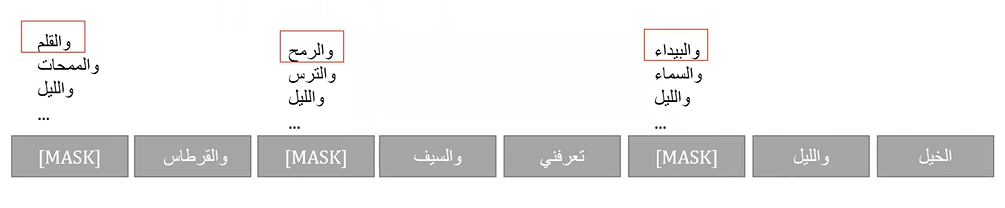
\includegraphics[scale=0.8]{Figures/arabert_example.PNG}
            %%     \caption{Different ways to use BERT.\cite{BERT}}
            %     \label{fig:cmp}
            % \end{figure}
            
            
            \begin{figure}[h]
                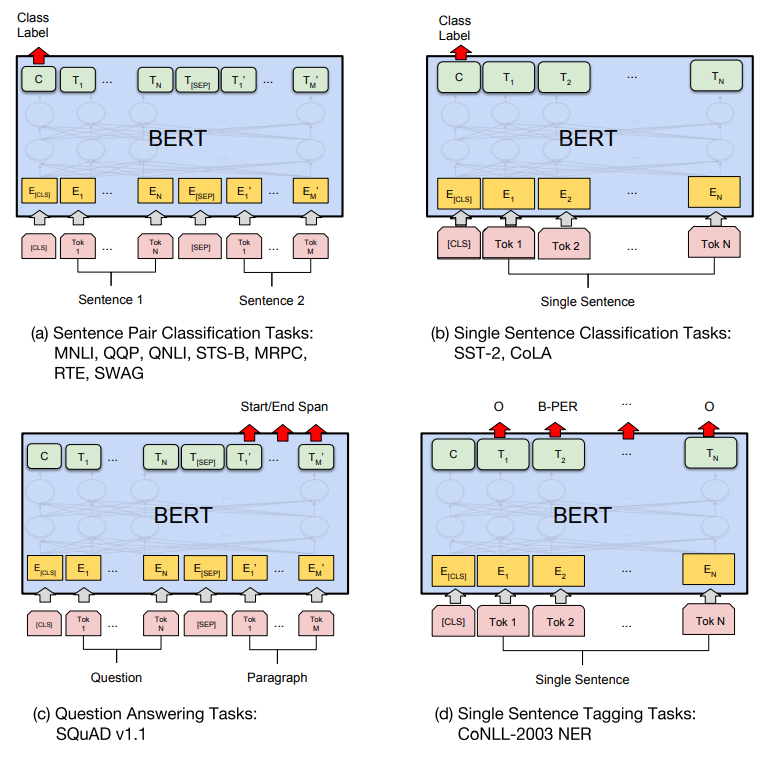
\includegraphics[scale=0.52]{Figures/BERT_uses.png}
                \caption{Different ways to use BERT.\cite{BERT}}
                \label{fig:different_ways_to_use_BERT}
            \end{figure}
            
            
            
            \subsubsection{Contextual Embeddings}
            % Computers can't understand normal text because it can only see it as a bunch of binary numbers and because of that it can't understand the meanings of words, so the solution to that is embeddings, embeddings works by assigning a unique vector of numbers to a specific word,  ideally an embedding captures some of the semantics of the text by placing semantically similar text close together in the embedding space, this works by finding what other words it often appears next to, so for example after finding the embeddings list or dictionary and you want to know what is the most similar words to \RL{العربية} you would have to calculate it's vector and other vectors distance in the list to measures the similarity and relationship between them.
            % Sorry, I shouldn't have let you write this. It isnt needed
            
            One problem traditional embeddings face is that it doesn't capture the contextual semantic information the word represents, for example \RL{ذهبنا الى البر ثم اكلنا خبز البر} here we used the word \RL{البر} in two contexts, traditional embeddings will represent those two words as the with the same vector, embeddings aware of the context they're in are known as contextual embeddings.
            
            
            The first architecture that implements this sort of idea is Embeddings from Language Models (\emph{ELMo}), which does this by taking the hidden layers of words that come before and after the word we want the embeddings for, then multiplying this the hidden layer by a weighing vector then adding the result to the original word's embedding, this essentially represents nudging the embedding towards the context the word is in.
            The same idea is also implemented by BERT.
            
            % The difference between normal embeddings and contextual embeddings is that the word embeddings capture word semantics in context such that it can represent differently under different context even though it is same word, one example of that is ELMo which BERT uses it internally.
            % Repeat of same info
            % BERT doesnt use ELMo
        
            
    
    \section{Experimental design}
    % Experimental design: includes all variables in experiment
    % Add brief two line intro if you think its needed
    
        \subsection{Datasets}
        In their final records, SMADC dataset contained 1,088,578 documents. which consisted of 812,849 Facebook comments, 9,440 online newspaper comments, and 266,289 Twitter tweets\cite{alshutayri}. And each one of them are distributed in the five labels (GLF, EGY, NOR, LEV and IRQ) The highest rate of the collected data was from Facebook comments as seen in Figure 9. Later on, they added more data to the dataset based on their previous steps of filtration.
        \begin{figure}[h]
            % \hskip-3.3cm
            \centering
            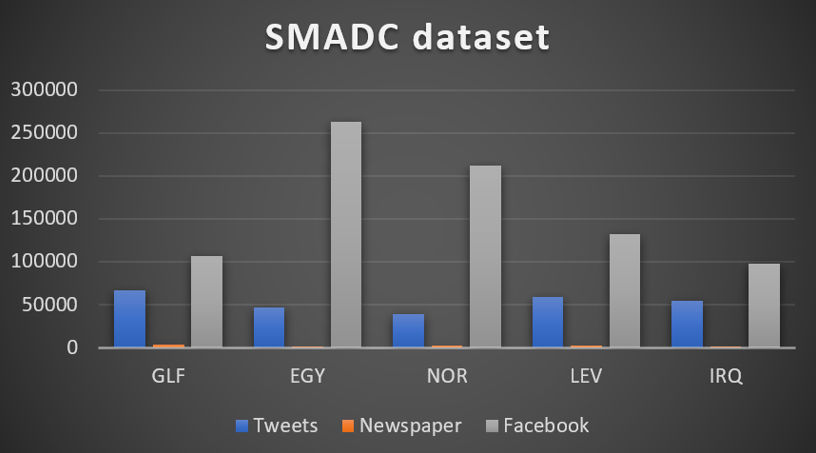
\includegraphics[scale=0.85]{Figures/SMADC dataset chart.PNG}
            \caption{SMADC dataset chart}
            \label{fig:cmp}
        \end{figure}
        
        % Overview of what does the SMADC dataset contain (numbers on how many records, their distribution (you can add a bar graph too))
        % Anything more you want to add
        
        \subsection{Algorithms}
        After the success of BERT and the growing development of machine learning models and state-of-art techniques, it has become important to implement a BERT model that understands the Arabic language. Wissam Antoun and others developed \emph{AraBERT}, they pre-trained BERT to be strongly focused on Arabic language and they managed to fulfill state-of-the-art performance by testing it on most Arabic NLP tasks. They covered 1.5 billion words from different medias and articles from diverse Arab countries.\cite{wissam}
        For the purposes of this research, we'll use their implementation of BERT.
        % In their pre-training they used the \emph{Masked Language Modeling} (MLM), which it requires to understand the left and right context without any labeled data by just using a raw text.  Small percentage of input tokens are selected for replacement. Those tokens are replaced 80\% with the [MASK] token, and 20\% either a random token or the original token\cite{wissam}.
        
        
        We've also introduced a warmup ratio which should accelerate our model to achieving optimality. The main idea is to use a variable learning rate increases linearly from a set minimum to a maximum then linearly decreases over the remaining number of steps. This will help us to decrease the amount of training hours and save our resources.
        
        
\bibliographystyle{plain} % We choose the &quot;plain&quot; reference style
\bibliography{cite.bib} % Entries are in the &quot;refs.bib&quot; file</code></pre>

\end{document}